% -*- root: Dissertation.tex -*-
\documentclass[Dissertation.tex]{subfiles}
\begin{document}
\graphicspath{{../Figures/}}
\chapter{Comparison of Primitive, Conservation, and Entropy Variables for Compressible Navier-Stokes}
\label{sec:VariableComparison}
% \section{Nonlinear Formulation}
In this appendix we discuss some work we did exploring a comparison between three formulations of the 
compressible Navier-Stokes equations: primitive variables, conservation variables, and entropy variables.

\section{Primitive Variables}
We begin by recalling the definitions for primitive variables:
\begin{align*}
C_c&:=\rho\\
\bfC_m&:=\rho\bfu\\
C_e&:=\rho(C_v T+\frac{1}{2}\bfu\cdot\bfu)\\
\bfF_c&:=\rho\bfu\\
\mathbb{F}_m&:=\rho\bfu\otimes\bfu+\rho RT\bbI\\
\bfF_e&:=\rho\bfu\LRp{C_v T+\frac{1}{2}\bfu\cdot\bfu}+\bfu\rho RT\\
\bfK_c&:=\boldsymbol 0\\
\bbK_m&:=\LRp{\bbD+\bbD^T-\frac{2}{3}\trace(\bbD)\bbI}\\
\bfK_e&:=-\bfq+\bfu\cdot\LRp{\bbD+\bbD^T-\frac{2}{3}\trace(\bbD)\bbI}\\
\bbM_{\bbD}&:=\bbD\\
\bfM_{\bfq}&:=\frac{Pr}{C_p}\bfq\\
\bfG_{\bbD}&:=\bfu\\
G_{\bfq}&:=-T\,.
\end{align*}

\subsection{Linearized Terms}
Now we introduce the linearized terms:
\begin{align*}
\pd{C_c(\tilde W)}{W}\Delta W&:=
	\Delta\rho\\
\pd{\bfC_m(\tilde W)}{W}\Delta W&:=
	\Delta\rho\tilde\bfu+\tilde\rho\Delta\bfu\\
\pd{C_e(\tilde W)}{W}\Delta W&:=
	C_v\Delta\rho\tilde T+C_v\tilde\rho\Delta T
	+\frac{1}{2}\LRp{\Delta\rho\tilde\bfu\cdot\tilde\bfu+\tilde\rho\Delta\bfu\cdot\tilde\bfu+\tilde\rho\tilde\bfu\cdot\Delta\bfu}\\
\pd{\bfF_c(\tilde W)}{W}\Delta W&:=
	\Delta\rho\tilde\bfu+\tilde\rho\Delta\bfu\\
\pd{\mathbb{F}_m(\tilde W)}{W}\Delta W&:=
	\Delta\rho\tilde\bfu\otimes\tilde\bfu
	+\tilde\rho\Delta\bfu\otimes\tilde\bfu
	+\tilde\rho\tilde\bfu\otimes\Delta\bfu
	+R\LRp{\Delta\rho\tilde T+\tilde\rho\Delta T}\bbI\\
\pd{\bfF_e(\tilde W)}{W}\Delta W&:=
	C_v\Delta\rho\tilde\bfu\tilde T+C_v\tilde\rho\Delta\bfu\tilde T+C_v\tilde\rho\tilde\bfu\Delta T
	\\&\quad
	+\frac{1}{2}\Delta\rho\tilde\bfu\tilde\bfu\cdot\tilde\bfu
	+\frac{1}{2}\tilde\rho\Delta\bfu\tilde\bfu\cdot\tilde\bfu
	+\frac{1}{2}\tilde\rho\tilde\bfu\Delta\bfu\cdot\tilde\bfu
	+\frac{1}{2}\tilde\rho\tilde\bfu\tilde\bfu\cdot\Delta\bfu
	\\&\quad
	+R\Delta\bfu\tilde\rho\tilde T
	+R\tilde\bfu\Delta\rho\tilde T
	+R\tilde\bfu\tilde\rho\Delta T\\
\pd{\bfK_c(\tilde W)}{W}\Delta W&:=
	\boldsymbol 0\\
\pd{\bbK_m(\tilde W)}{W}\Delta W&:=
	\LRp{\Delta\bbD+\Delta\bbD^T-\frac{2}{3}\trace(\Delta\bbD)\bbI}\\
\pd{\bfK_e(\tilde W)}{W}\Delta W&:=
	-\Delta\bfq+\Delta\bfu\cdot\LRp{\tilde\bbD+\tilde\bbD^T-\frac{2}{3}\trace(\tilde\bbD)\bbI}
	\\&\quad
	+\tilde\bfu\cdot\LRp{\Delta\bbD+\Delta\bbD^T-\frac{2}{3}\trace(\Delta\bbD)\bbI}\\
\pd{\bbM_{\bbD}(\tilde W)}{W}\Delta W&:=
	\Delta\bbD\\
\pd{\bfM_{\bfq}(\tilde W)}{W}\Delta W&:=
	\frac{Pr}{C_p}\Delta\bfq\\
\pd{\bfG_{\bbD}(\tilde W)}{W}\Delta W&:=
	\Delta\bfu\\
\pd{G_{\bfq}(\tilde W)}{W}\Delta W&:=
	-\Delta T\,.
\end{align*}

\section{Conservation Variables}
Now we wish to do a change of variables to conservation variables: 
\begin{align*}
\rho&=\rho\\
\bfm&=\rho\bfu\\
E&=\rho\LRp{C_v T+\frac{1}{2}\bfu\cdot\bfu}
\end{align*}

\begin{align*}
C_c&:=\rho\\
\bfC_m&:=\bfm\\
C_e&:=E\\
\bfF_c&:=\bfm\\
\mathbb{F}_m&=\frac{\bfm\otimes\bfm}{\rho}+(\gamma-1)\LRp{E-\frac{\bfm\cdot\bfm}{2\rho}}\bbI\\
\bfF_e&=\gamma E\frac{\bfm}{\rho}-(\gamma-1)\frac{\bfm\cdot\bfm}{2\rho^2}\bfm\\
\bfK_c&:=\boldsymbol 0\\
\bbK_m&:=\LRp{\bbD+\bbD^T-\frac{2}{3}\trace(\bbD)\bbI}\\
\bfK_e&:=-\bfq+\frac{\bfm}{\rho}\cdot\LRp{\bbD+\bbD^T-\frac{2}{3}\trace(\bbD)\bbI}\\
\bbM_{\bbD}&:=\bbD\\
\bfM_{\bfq}&:=\frac{Pr}{C_p}\bfq\\
\bfG_{\bbD}&:=\frac{\bfm}{\rho}\\
G_{\bfq}&:=-\LRp{\frac{E-\frac{1}{2\rho}\bfm\cdot\bfm}{C_v\rho}}\,.
\end{align*}

\subsection{Linearized Terms}
\begin{align*}
\pd{C_c(\tilde W)}{W}\Delta W&:=
	\Delta\rho\\
\pd{\bfC_m(\tilde W)}{W}\Delta W&:=
	\Delta\bfm\\
\pd{C_e(\tilde W)}{W}\Delta W&:=
	\Delta E\\
\pd{\bfF_c(\tilde W)}{W}\Delta W&:=
	\Delta\bfm\\
\pd{\mathbb{F}_m(\tilde W)}{W}\Delta W&:=
	\frac{\Delta\bfm\otimes\tilde\bfm}{\tilde\rho}
	+\frac{\tilde\bfm\otimes\Delta\bfm}{\tilde\rho}
	-\frac{\tilde\bfm\otimes\tilde\bfm}{\tilde\rho^2}\Delta\rho
	\\&\quad
	+(\gamma-1)\LRp{\Delta E
	-\frac{\Delta\bfm\cdot\tilde\bfm}{2\tilde\rho}
	-\frac{\tilde\bfm\cdot\Delta\bfm}{2\tilde\rho}
	+\frac{\tilde\bfm\cdot\tilde\bfm}{2\tilde\rho^2}\Delta\rho
	}\bbI\\
\pd{\bfF_e(\tilde W)}{W}\Delta W&:=
	\gamma\LRp{
	\Delta E\frac{\tilde\bfm}{\tilde\rho}
	+\tilde E\frac{\Delta\bfm}{\tilde\rho}
	-\tilde E\frac{\tilde\bfm}{\tilde\rho^2}\Delta\rho}
	\\&\quad
	+(\gamma-1)\left(
	-\frac{\Delta\bfm\tilde\bfm\cdot\tilde\bfm}{2\tilde\rho^2}
	-\frac{\tilde\bfm\Delta\bfm\cdot\tilde\bfm}{2\tilde\rho^2}
	\right.\\&\quad\quad\left.
	-\frac{\tilde\bfm\tilde\bfm\cdot\Delta\bfm}{2\tilde\rho^2}
	+\frac{\tilde\bfm\tilde\bfm\cdot\tilde\bfm}{\tilde\rho^3}\Delta\rho\right)\\
\pd{\bfK_c(\tilde W)}{W}\Delta W&:=
	\boldsymbol 0\\
\pd{\bbK_m(\tilde W)}{W}\Delta W&:=
	\LRp{\Delta\bbD+\Delta\bbD^T-\frac{2}{3}\trace(\Delta\bbD)\bbI}\\
\pd{\bfK_e(\tilde W)}{W}\Delta W&:=
	-\Delta\bfq+\LRp{\frac{\Delta\bfm}{\tilde\rho}-\frac{\tilde\bfm}{\tilde\rho^2}\Delta\rho}
	\cdot\LRp{\tilde\bbD+\tilde\bbD^T-\frac{2}{3}\trace(\tilde\bbD)\bbI}
	\\&\quad
	+\frac{\tilde\bfm}{\tilde\rho}\cdot\LRp{\Delta\bbD+\Delta\bbD^T-\frac{2}{3}\trace(\Delta\bbD)\bbI}\\
\end{align*}
\begin{align*}
\pd{\bbM_{\bbD}(\tilde W)}{W}\Delta W&:=
	\Delta\bbD\\
\pd{\bfM_{\bfq}(\tilde W)}{W}\Delta W&:=
	\frac{Pr}{C_p}\Delta\bfq\\
\pd{\bfG_{\bbD}(\tilde W)}{W}\Delta W&:=
	\frac{\Delta\bfm}{\tilde\rho}-\frac{\tilde\bfm}{\tilde\rho^2}\Delta\rho\\
\pd{G_{\bfq}(\tilde W)}{W}\Delta W&:=
	-\left(\frac{\Delta E-\frac{1}{2\tilde\rho}\Delta\bfm\cdot\tilde\bfm
	-\frac{1}{2\tilde\rho}\tilde\bfm\cdot\Delta\bfm
	+\frac{1}{2\tilde\rho^2}\tilde\bfm\cdot\tilde\bfm\Delta\rho}{C_v\tilde\rho}
	\right.\\&\quad\left.
	-\frac{\tilde E-\frac{1}{2\tilde\rho}\tilde\bfm\cdot\tilde\bfm}{C_v\tilde\rho^2}\Delta\rho\right)
\,.
\end{align*}

\section{Entropy Variables}
Now we wish to do a change of variables to entropy variables:
\begin{align*}
V_c&=\frac{-E+(E-\frac{1}{2\rho}\bfm\cdot\bfm)\LRp{\gamma+1-\ln\LRs{\frac{(\gamma-1)(E-\frac{1}{2\rho}\bfm\cdot\bfm)}{\rho^\gamma}}}}
{E-\frac{1}{2\rho}\bfm\cdot\bfm}\\
\bfV_m&=\frac{\bfm}{E-\frac{1}{2\rho}\bfm\cdot\bfm}\\
V_e&=\frac{-\rho}{E-\frac{1}{2\rho}\bfm\cdot\bfm}\\
\end{align*}
with reverse mapping:
\begin{align*}
\rho&=-\alpha V_e\\
\bfm&=\alpha\bfV_m\\
E&=\alpha\LRp{1-\frac{1}{2V_e}\bfV_m\cdot\bfV_m}\\
\end{align*}
where 
\[
\alpha(V_c,\bfV_m,V_e)=\LRs{\frac{\gamma-1}{(-V_e)^\gamma}}^{\frac{1}{\gamma-1}}\exp\LRs{\frac{-\gamma+V_c-\frac{1}{2V_e}\bfV_m\cdot\bfV_m}{\gamma-1}}
\]

\begin{align*}
C_c&:=-\alpha V_e\\
\bfC_m&:=\alpha\bfV_m\\
C_e&:=\alpha\LRp{1-\frac{1}{2V_e}\bfV_m\cdot\bfV_m}\\
\bfF_c&=\alpha\bfV_m\\
\mathbb{F}_m&=\alpha\LRp{-\frac{\bfV_m\otimes\bfV_m}{V_e}+(\gamma-1)\bbI}\\
\bfF_e&=\alpha\frac{\bfV_m}{V_e}\LRp{\frac{1}{2V_e}\bfV_m\cdot\bfV_m-\gamma}\\
\bfK_c&:=\boldsymbol 0\\
\bbK_m&:=\LRp{\bbD+\bbD^T-\frac{2}{3}\trace(\bbD)\bbI}\\
\bfK_e&:=-\bfq+\frac{\bfV_m}{V_e}\cdot\LRp{\bbD+\bbD^T-\frac{2}{3}\trace(\bbD)\bbI}\\
\bbM_{\bbD}&:=\bbD\\
\bfM_{\bfq}&:=\frac{Pr}{C_p}\bfq\\
\bfG_{\bbD}&:=-\frac{\bfV_m}{V_e}\\
G_{\bfq}&:=\frac{1}{C_vV_e}\,.
\end{align*}

\subsection{Linearized Terms}
\begin{align*}
\pd{C_c(\tilde W)}{W}\Delta W&:=
	-\tilde V_e\pd{\alpha(\tilde W)}{W}\Delta W-\alpha(\tilde W)\Delta V_e
	\\
\pd{\bfC_m(\tilde W)}{W}\Delta W&:=
	\tilde\bfV_m\pd{\alpha(\tilde W)}{W}\Delta W+\alpha(\tilde W)\Delta\bfV_m
	\Delta\rho\tilde\bfu+\tilde\rho\Delta\bfu
	\\
\pd{C_e(\tilde W)}{W}\Delta W&:=
	\LRp{1-\frac{1}{2\tilde V_e}\tilde\bfV_m\cdot\tilde\bfV_m}\pd{\alpha(\tilde W)}{W}\Delta W
	\\&\quad
	-\alpha(\tilde W)\frac{1}{\tilde V_e}\tilde\bfV_m\cdot\Delta\bfV_m
	+\alpha(\tilde W)\frac{1}{2\tilde V_e^2}\tilde\bfV_m\cdot\tilde\bfV_m\Delta V_e
	\\
\pd{\bfF_c(\tilde W)}{W}\Delta W&:=
	\tilde\bfV_m\pd{\alpha(\tilde W)}{W}\Delta W+\alpha(\tilde W)\Delta\bfV_m
	\\
\pd{\mathbb{F}_m(\tilde W)}{W}\Delta W&:=
	\LRp{-\frac{\tilde\bfV_m\otimes\tilde\bfV_m}{\tilde V_e}+(\gamma-1)\bbI}\pd{\alpha(\tilde W)}{W}\Delta W
	\\&\quad
	+\alpha(\tilde W)\LRp{
	-\frac{\Delta\bfV_m\otimes\tilde\bfV_m}{\tilde V_e}
	-\frac{\tilde\bfV_m\otimes\Delta\bfV_m}{\tilde V_e}
	+\frac{\tilde\bfV_m\otimes\tilde\bfV_m}{\tilde V_e^2}\Delta V_e
	}
	\\
\pd{\bfF_e(\tilde W)}{W}\Delta W&:=
	\frac{\tilde\bfV_m}{\tilde V_e}
	\LRp{\frac{1}{2\tilde V_e}\tilde\bfV_m\cdot\tilde\bfV_m-\gamma}\pd{\alpha(\tilde W)}{W}\Delta W
	\\&\quad
	+\alpha(\tilde W)\left(
	\frac{\Delta\bfV_m}{\tilde V_e}\LRp{\frac{1}{2\tilde V_e}\tilde\bfV_m\cdot\tilde\bfV_m-\gamma}
	\right.\\&\quad\quad\left.
	-\frac{\tilde\bfV_m}{V_e^2}\LRp{\frac{1}{2\tilde V_e}\tilde\bfV_m\cdot\tilde\bfV_m-\gamma}\Delta V_e
	\right.\\&\quad\quad\left.
	+\frac{\tilde\bfV_m}{\tilde V_e}\LRp{
	\frac{1}{\tilde V_e}\tilde\bfV_m\cdot\Delta\bfV_m
	-\frac{1}{2\tilde V_e^2}\tilde\bfV_m\cdot\tilde\bfV_m\Delta V_e
	}
	\right)
	\\
\end{align*}
\begin{align*}
\pd{\bfK_c(\tilde W)}{W}\Delta W&:=
	\boldsymbol 0\\
\pd{\bbK_m(\tilde W)}{W}\Delta W&:=
	\LRp{\Delta\bbD+\Delta\bbD^T-\frac{2}{3}\trace(\Delta\bbD)\bbI}
	\\
\pd{\bfK_e(\tilde W)}{W}\Delta W&:=
	-\Delta\bfq+
	\LRp{\frac{\Delta\bfV_m}{\tilde V_e}-\frac{\tilde\bfV_m}{\tilde V_e^2}\Delta V_e}
	\cdot\LRp{\tilde\bbD+\tilde\bbD^T-\frac{2}{3}\trace(\tilde\bbD)\bbI}
	\\&\quad
	+\frac{\tilde\bfV_m}{\tilde V_e}\cdot\LRp{\Delta\bbD+\Delta\bbD^T-\frac{2}{3}\trace(\Delta\bbD)\bbI}\\
\pd{\bbM_{\bbD}(\tilde W)}{W}\Delta W&:=
	\Delta\bbD
	\\
\pd{\bfM_{\bfq}(\tilde W)}{W}\Delta W&:=
	\frac{Pr}{C_p}\Delta\bfq
	\\
\pd{\bfG_{\bbD}(\tilde W)}{W}\Delta W&:=
	-\LRp{\frac{\Delta\bfV_m}{\tilde V_e}-\frac{\tilde\bfV_m}{\tilde V_e^2}\Delta V_e}
	\\
\pd{G_{\bfq}(\tilde W)}{W}\Delta W&:=
	-\frac{1}{C_vV_e^2}\Delta V_e
	\,.
\end{align*}
\begin{align*}
\pd{\alpha(\tilde W)}{W}\Delta W&=
\LRs{\frac{\gamma-1}{(-\tilde V_e)^\gamma}}^{\frac{2-\gamma}{\gamma-1}}
\gamma(-\tilde V_e)^{-(\gamma+1)}
\exp\LRs{\frac{-\gamma+\tilde V_c-\frac{1}{2\tilde V_e}\tilde\bfV_m\cdot\tilde\bfV_m}{\gamma-1}}
\Delta V_e\\
&+\LRs{\frac{\gamma-1}{(-\tilde V_e)^\gamma}}^{\frac{1}{\gamma-1}}
\exp\LRs{\frac{-\gamma+\tilde V_c-\frac{1}{2\tilde V_e}\tilde\bfV_m\cdot\tilde\bfV_m}{\gamma-1}}
\frac{1}{\gamma-1}\\
&\LRp{\Delta V_c
-\frac{1}{\tilde V_e}\tilde\bfV_m\cdot\Delta\bfV_m
+\frac{1}{2\tilde V_e^2}\tilde\bfV_m\cdot\tilde\bfV_m\Delta V_e
}
\end{align*}


\section{Numerical Experiments}
We perform a couple numerical experiments to compare the different formulations.
In Chapter \ref{sec:compressible} we used a incrementally decreased $\mu$ with ever refinement step 
as this approach was found to produce cleaner refinement patterns; here we hold $\mu$ constant
for each problem to show that it is still possible to arrive at a converged solution, but
we end up with a less desirable final refinement pattern.

\subsection{Sod Shock Tube}
% Re=1e5, p=2, delta_p=2, nlMaxIters=10, NSDecoupled
We repeat the Sod shock tube problem described in Chapter \ref{sec:compressible} with $\mu=10^{-5}$,
$p=2$, $\Delta p=2$, and the NSDecoupled norm.
We omit plots of velocity and pressure as they don't really contribute anything new to the comparisons.
Comparing figures (\ref{fig:SodPrimitive} - \ref{fig:SodEntropy}), it seems that
primitive and entropy variables are of similiar quality, at least by the eyeball norm.
Entropy variables, on the other hand, suffer from much more extreme overshoots and 
undershoots compared to the other formulations.

\begin{figure}[ht]
\centering
\begin{subfigure}[t]{\textwidth}
\centering
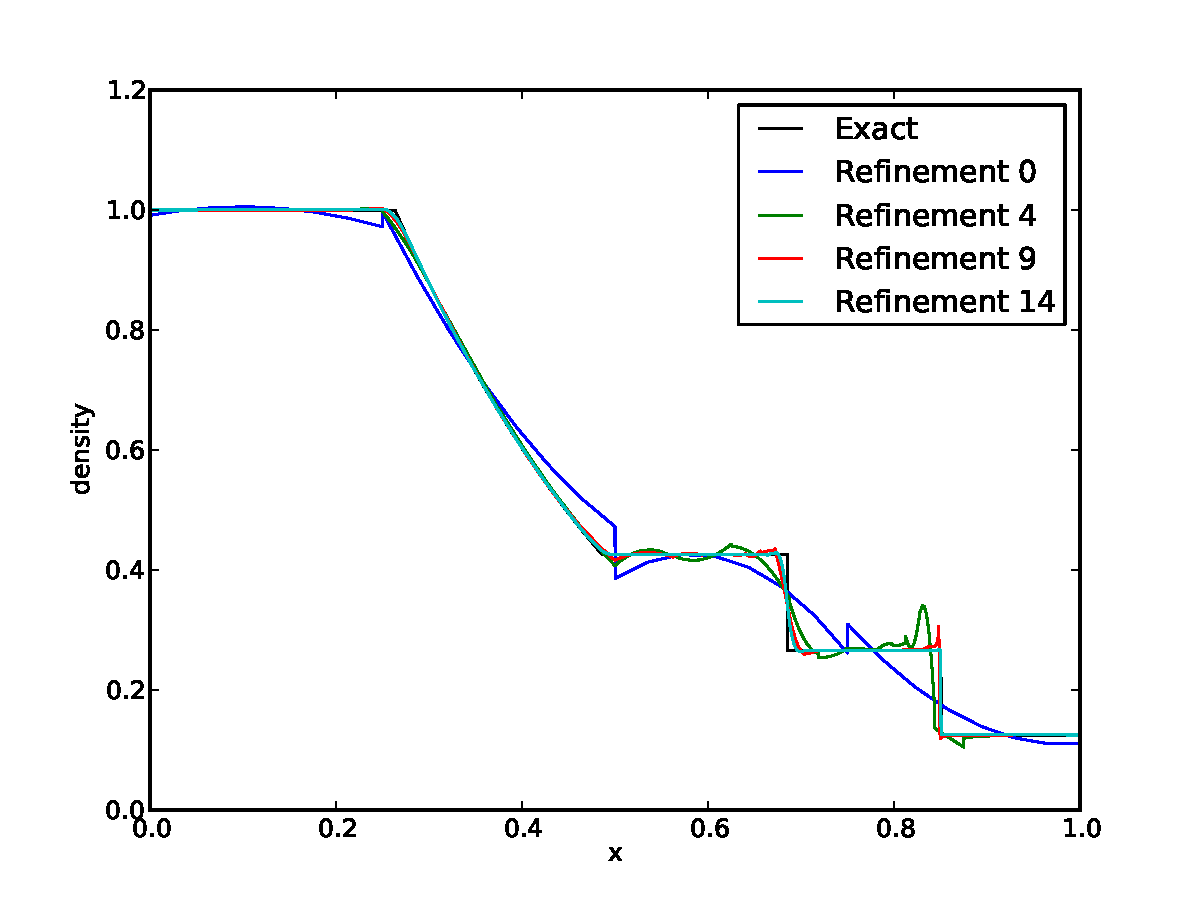
\includegraphics[width=\textwidth]{Dissertation/Sod/FormulationComparison/primitive-den.pdf}
\caption{Density}
\end{subfigure}
% \begin{subfigure}[t]{0.7\textwidth}
% \centering
% 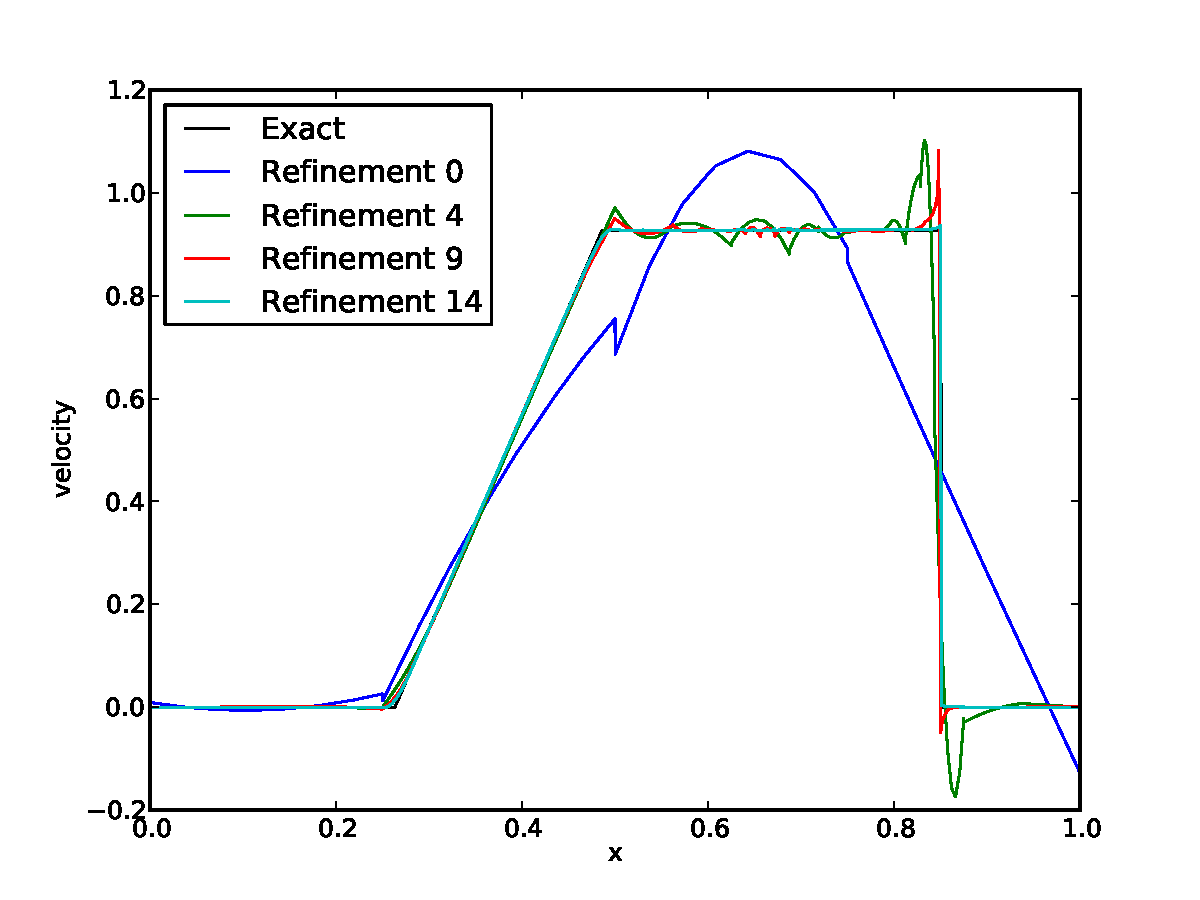
\includegraphics[width=\textwidth]{Dissertation/Sod/FormulationComparison/primitive-vel.pdf}
% \caption{Velocity}
% \end{subfigure}
% \begin{subfigure}[t]{0.7\textwidth}
% \centering
% 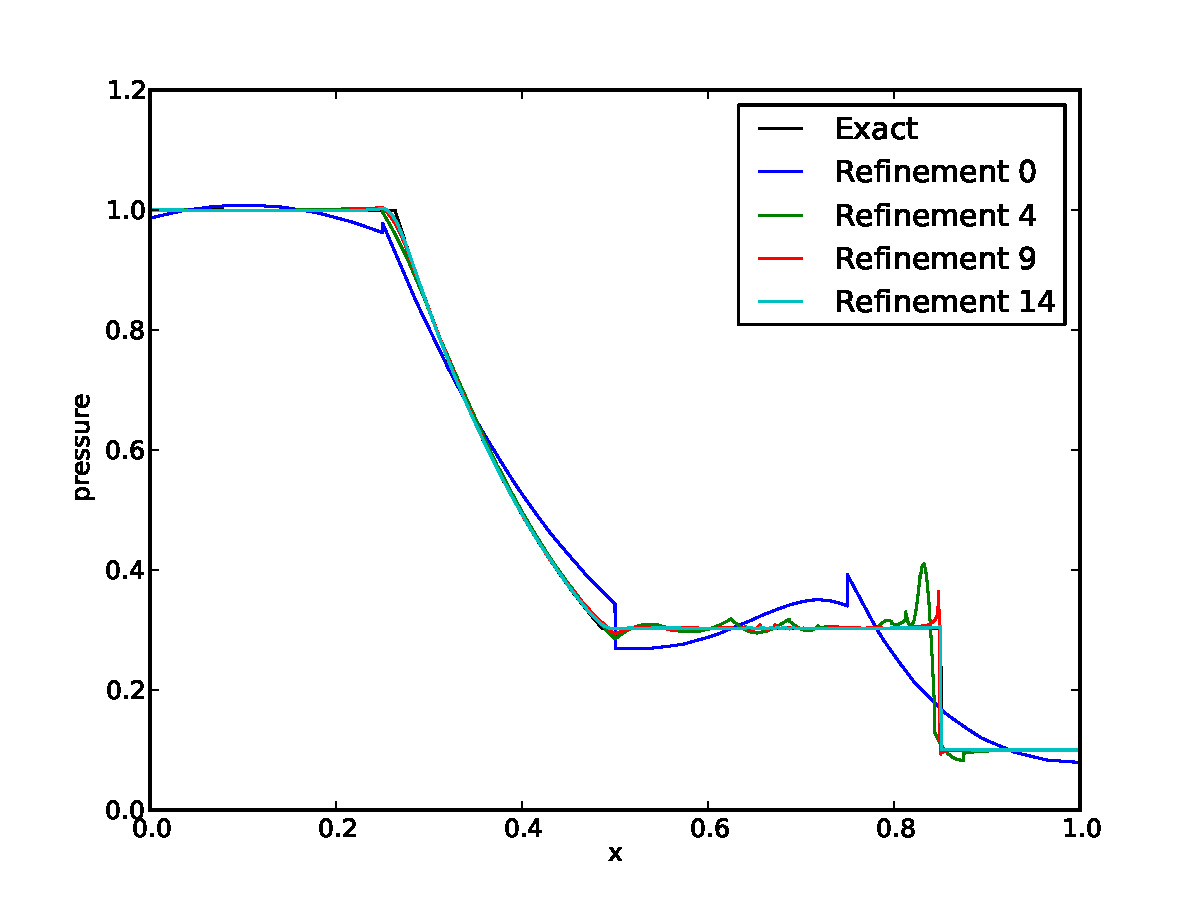
\includegraphics[width=\textwidth]{Dissertation/Sod/FormulationComparison/primitive-pres.pdf}
% \caption{Pressure}
% \end{subfigure}
\begin{subfigure}[t]{0.9\textwidth}
\centering
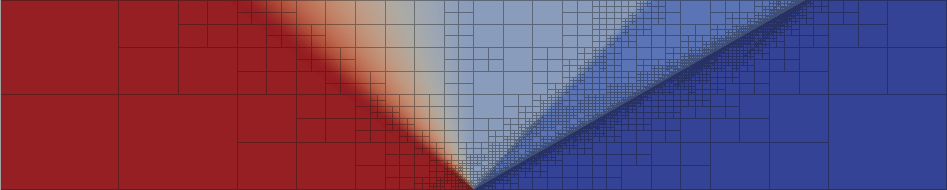
\includegraphics[width=\textwidth]{Sod/FormulationComparison/Form0Mesh15.png}
\caption{Final mesh colored by $\rho$}
\end{subfigure}
\caption{Sod problem with primitive variables}
\label{fig:SodPrimitive}
\end{figure}

\begin{figure}[ht]
\centering
\begin{subfigure}[t]{\textwidth}
\centering
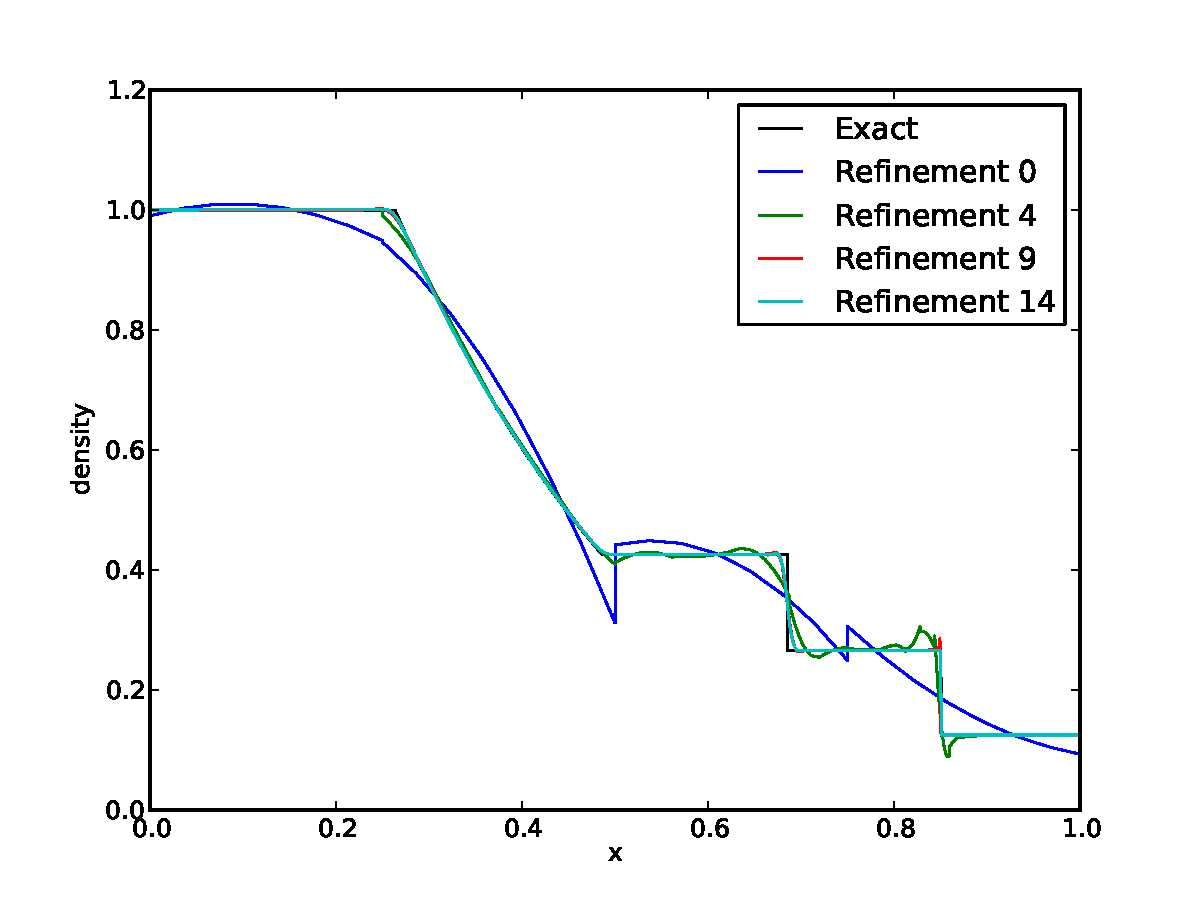
\includegraphics[width=\textwidth]{Dissertation/Sod/FormulationComparison/conservation-den.pdf}
\caption{Density}
\end{subfigure}
% \begin{subfigure}[t]{0.7\textwidth}
% \centering
% 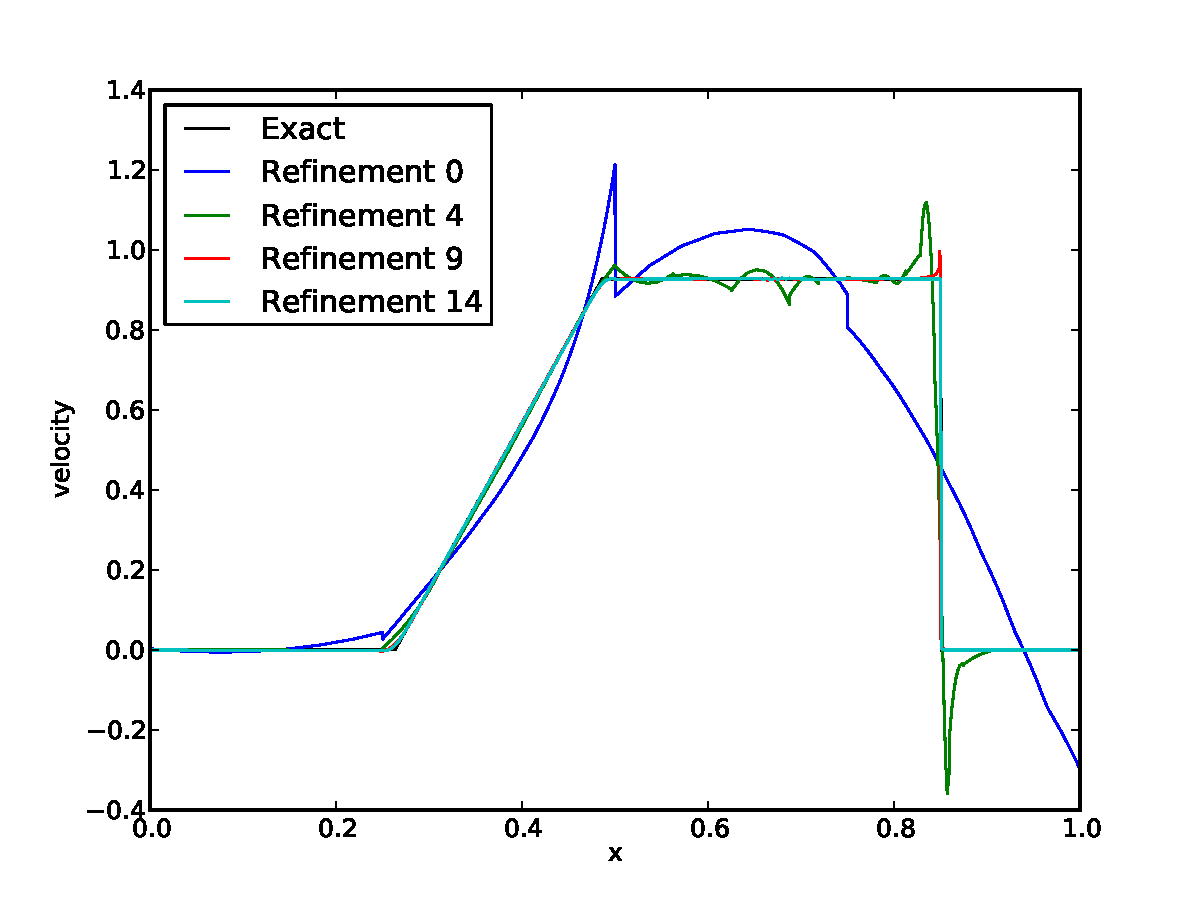
\includegraphics[width=\textwidth]{Dissertation/Sod/FormulationComparison/conservation-vel.pdf}
% \caption{Velocity}
% \end{subfigure}
% \begin{subfigure}[t]{0.7\textwidth}
% \centering
% 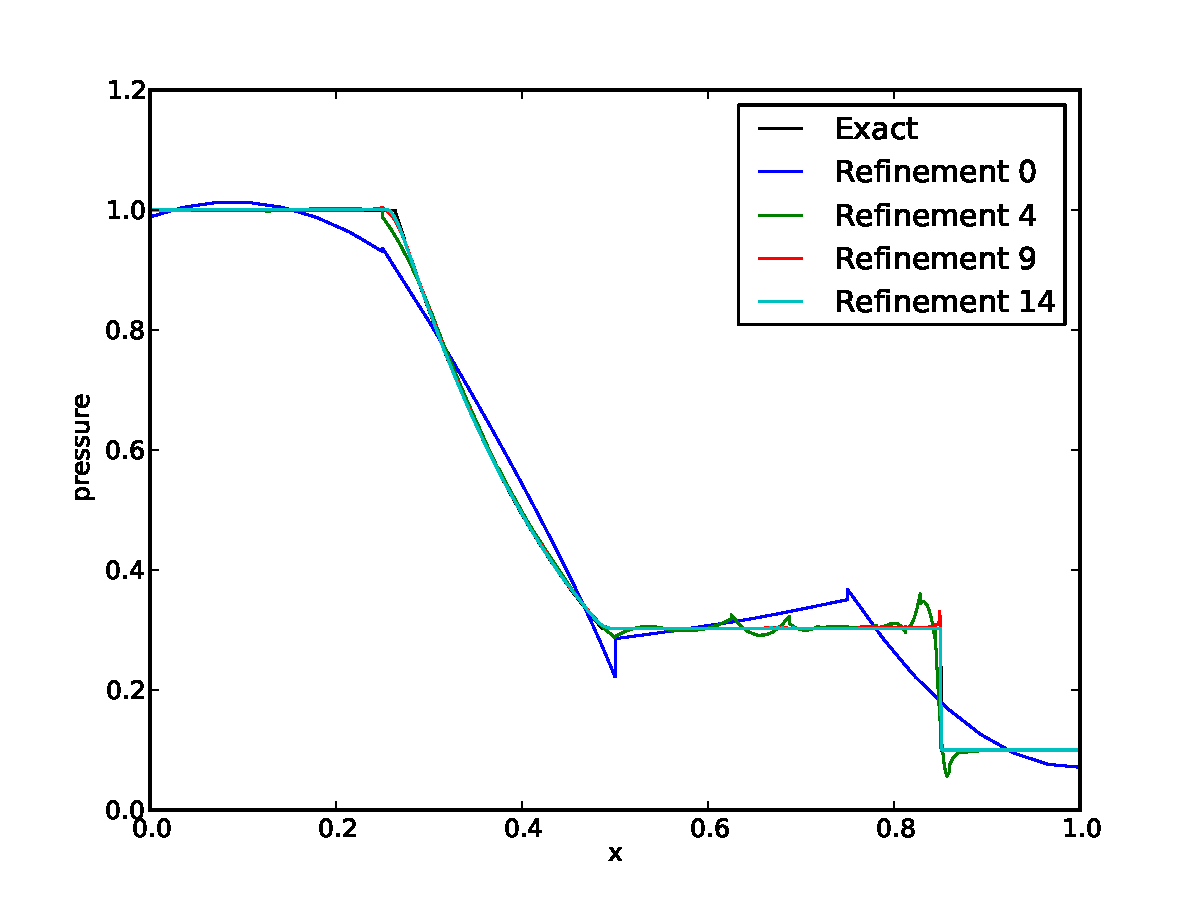
\includegraphics[width=\textwidth]{Dissertation/Sod/FormulationComparison/conservation-pres.pdf}
% \caption{Pressure}
% \end{subfigure}
\begin{subfigure}[t]{0.9\textwidth}
\centering
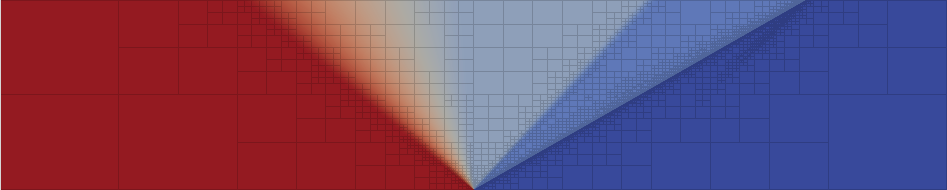
\includegraphics[width=\textwidth]{Sod/FormulationComparison/Form1Mesh15.png}
\caption{Final mesh colored by $\rho$}
\end{subfigure}
\caption{Sod problem with conservation variables}
\label{fig:SodConservation}
\end{figure}

\begin{figure}[ht]
\centering
\begin{subfigure}[t]{\textwidth}
\centering
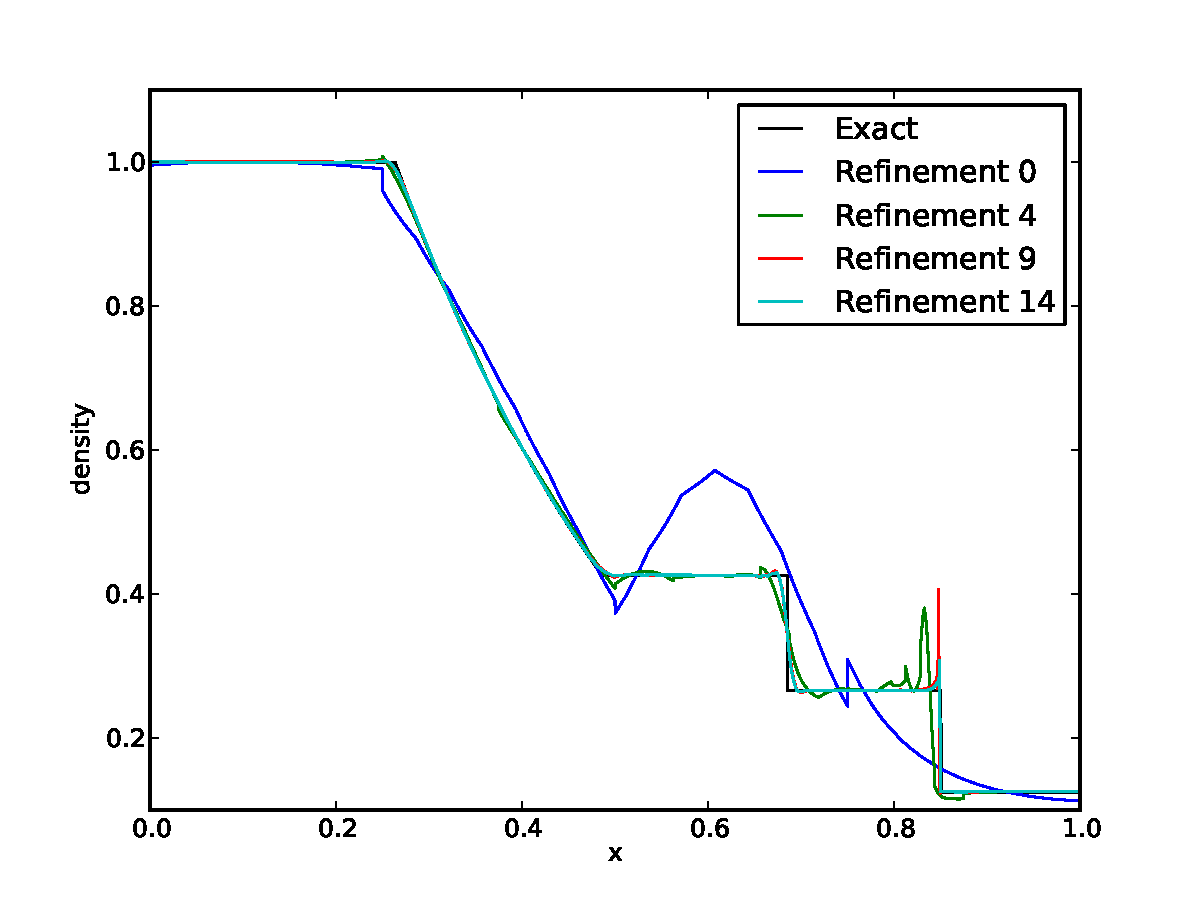
\includegraphics[width=\textwidth]{Dissertation/Sod/FormulationComparison/entropy-den.pdf}
\caption{Density}
\end{subfigure}
% \begin{subfigure}[t]{0.7\textwidth}
% \centering
% 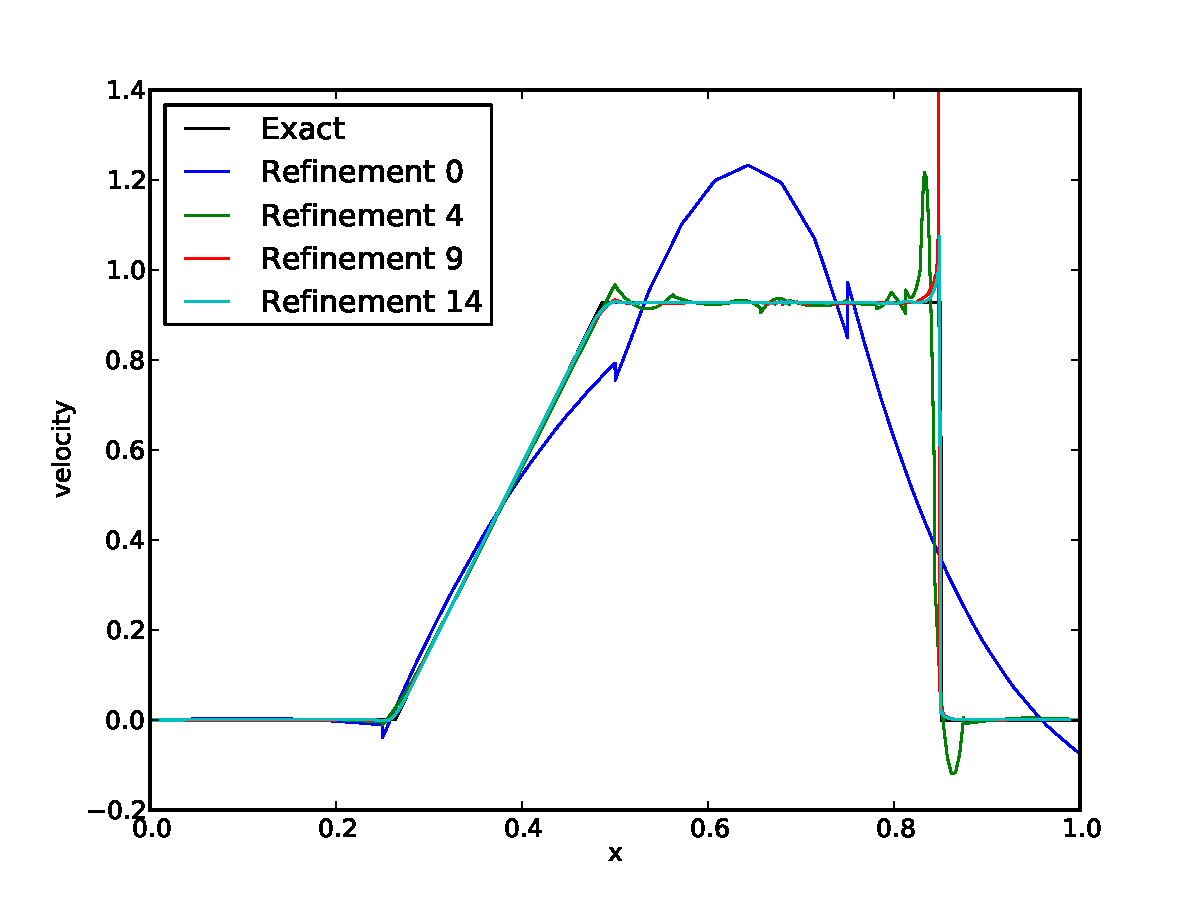
\includegraphics[width=\textwidth]{Dissertation/Sod/FormulationComparison/entropy-vel.pdf}
% \caption{Velocity}
% \end{subfigure}
% \begin{subfigure}[t]{0.7\textwidth}
% \centering
% 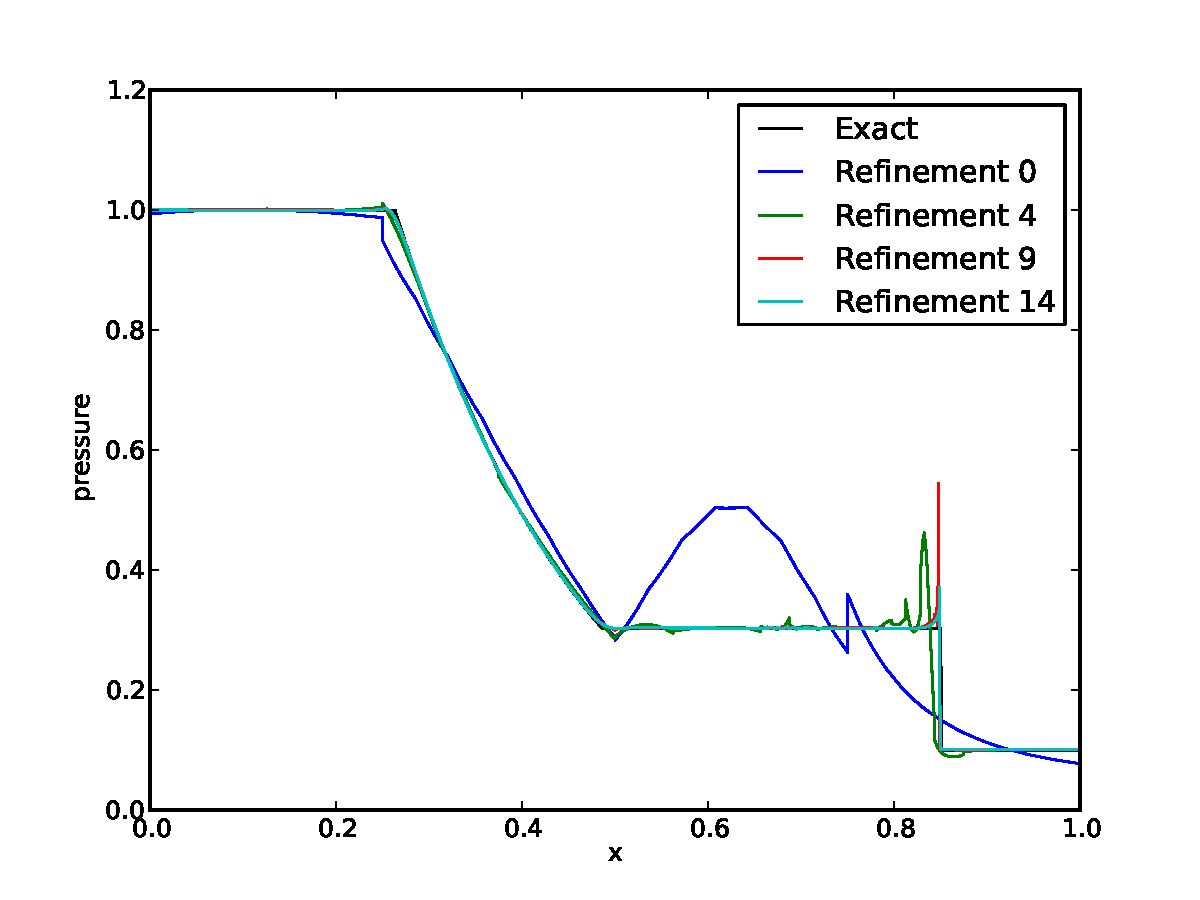
\includegraphics[width=\textwidth]{Dissertation/Sod/FormulationComparison/entropy-pres.pdf}
% \caption{Pressure}
% \end{subfigure}
\begin{subfigure}[t]{0.9\textwidth}
\centering
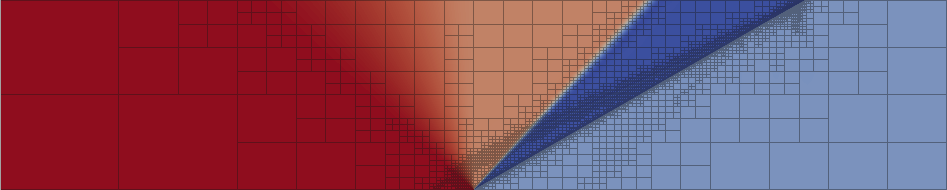
\includegraphics[width=\textwidth]{Sod/FormulationComparison/Form2Mesh15.png}
\caption{Final mesh colored by $V_c$}
\end{subfigure}
\caption{Sod problem with entropy variables}
\label{fig:SodEntropy}
\end{figure}

\subsection{Noh Implosion}
% Re=1e3, p=2, delta_p=2, nlMaxIters=10, timeslabs
We repeat the Noh problem from before with $\mu=10^{-3}$, $p=2$, $\Delta p=2$, and the NSDecoupled norm.
In Chapter \ref{sec:compressible} we simulated a half domain with a symmetry boundary condition
at the origin; here we compute the full domain.
The other difference is that this simulation was computed as a series of four time slabs 
rather than as one monolithic computation.
This means that the $[0,\frac{1}{4}]$ time slab was computed for 8 adaptive refinement steps
then the final solution was projected onto the $[\frac{1}{4},\frac{1}{2}]$ time slab as an 
initial condition.
This was repeated until we arrived at the $[\frac{3}{4},1]$ time slab, where the density traces
in Figure \ref{fig:NohDen} are taken.
We see more unwanted refinements in this computation compared to Chapter \ref{sec:compressible}
due to the spurious shock patterns that develop on coarse meshes.
We are not able to compare the entropy formulation for this problem since the initial conditions 
contain infinities under this formulation.

\begin{figure}[ht]
\centering
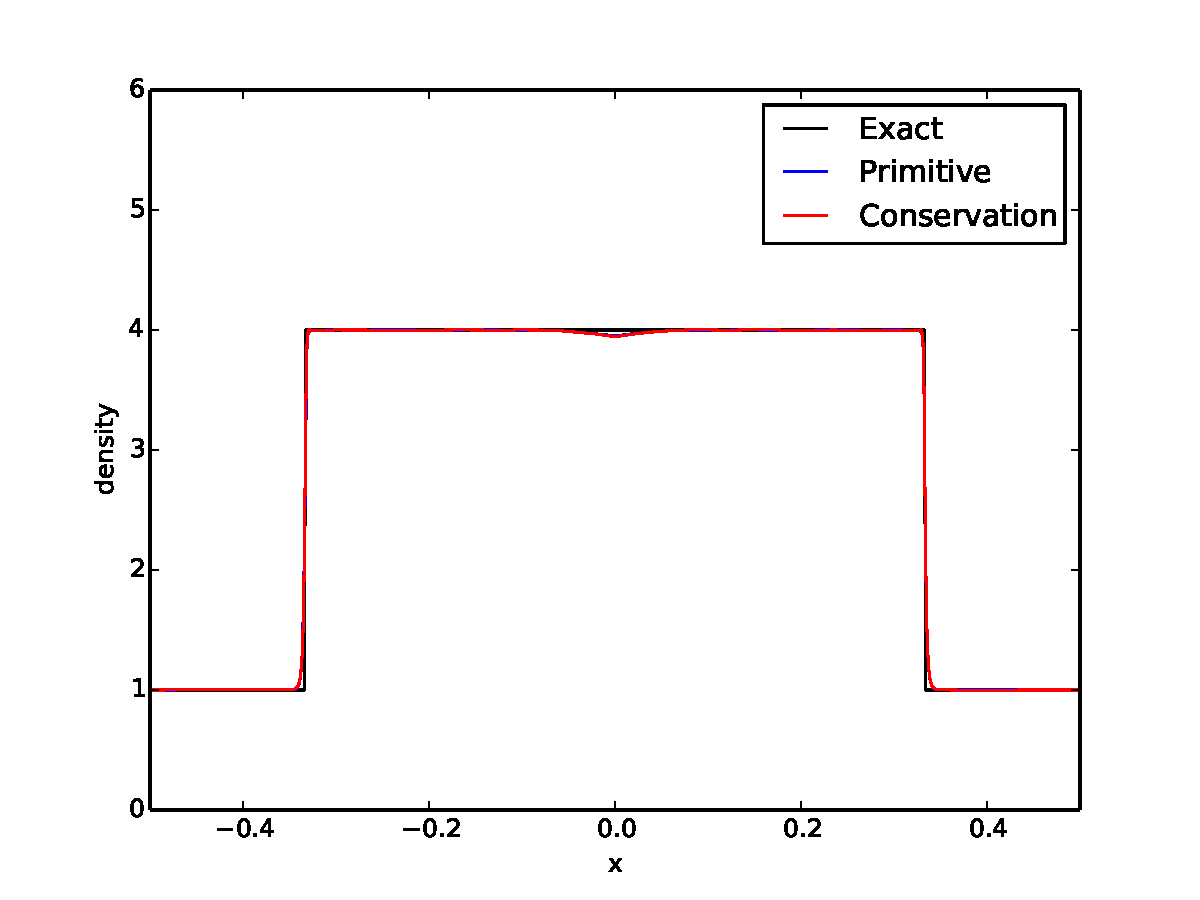
\includegraphics[width=\textwidth]{Noh/FormulationComparison/den9.pdf}
\caption{Density at final time}
\label{fig:NohDen}
\end{figure}

\begin{figure}[ht]
\centering
\begin{subfigure}[t]{0.9\textwidth}
\centering
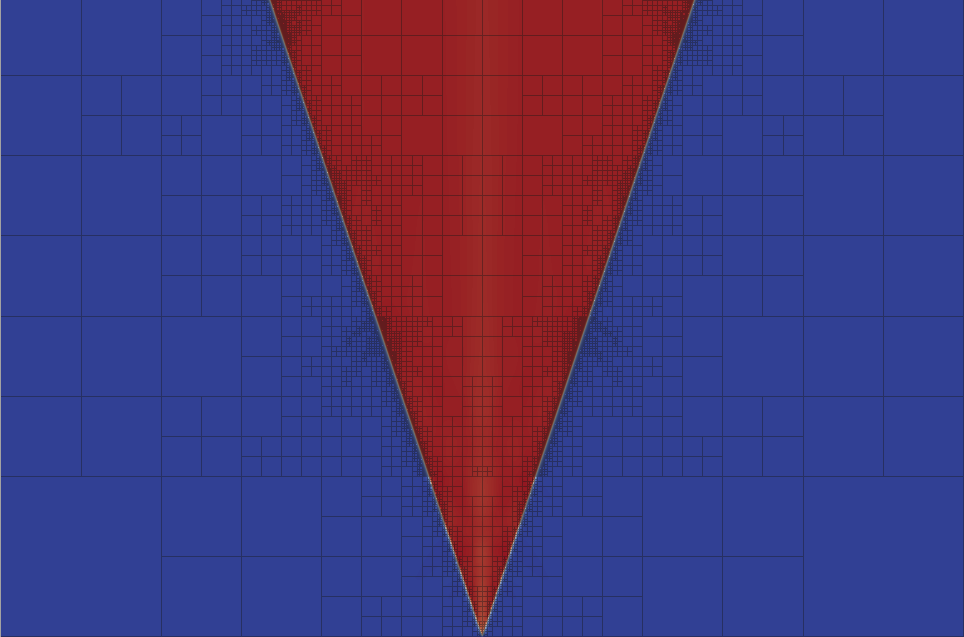
\includegraphics[width=\textwidth]{Noh/FormulationComparison/Form0Mesh8.png}
\caption{Final mesh with primitive variables}
\end{subfigure}
\begin{subfigure}[t]{0.9\textwidth}
\centering
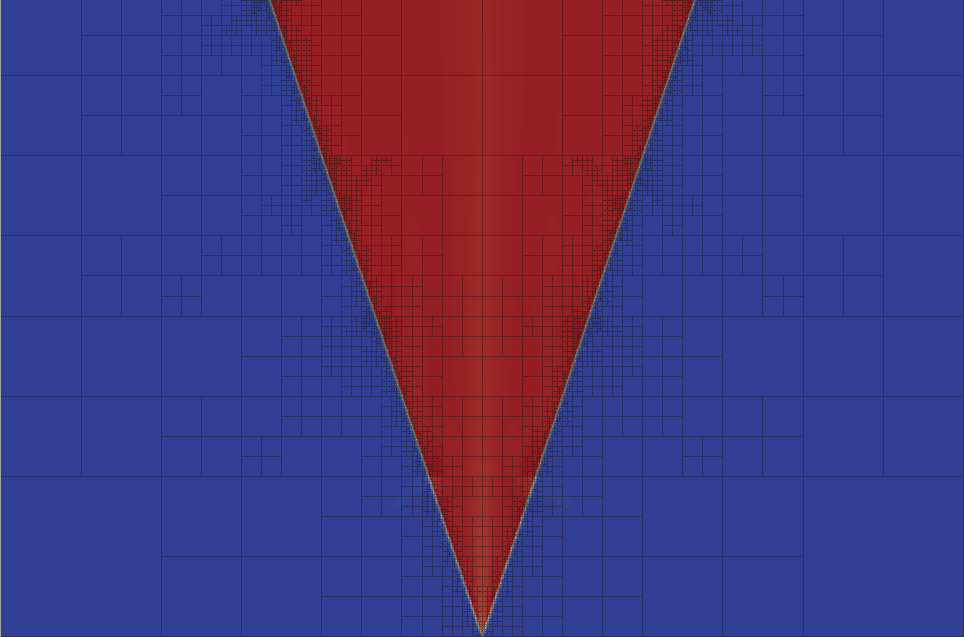
\includegraphics[width=\textwidth]{Noh/FormulationComparison/Form1Mesh8.png}
\caption{Final mesh with conservation variables}
\end{subfigure}
\caption{Noh meshes colored by $\rho$}
\label{fig:Noh}
\end{figure}

\end{document}
